\begin{abstract}
Modern software systems often exhibit configuration options to meet customer requirements, including a system's performance behavior. Performance models derived via machine learning are an established approach for estimating and optimizing configuration-dependent software performance.

Most existing approaches in this area rely on software performance measurements conducted with a single workload (i.e., input fed to a system). This single workload, however,  is often not representative of a software system's real-world application scenarios. Understanding to what extent configuration and
workload---individually and combined---cause a software system's performance to vary is key to understand whether performance
models are generalizable across different configurations and workloads. 
Yet, so far, this aspect has not been \textit{systematically}~studied.

To fill this gap, we conducted a systematic empirical study across 25\,258 configurations from nine real-world configurable software systems to investigate the effects of workload variation at system-level performance and for individual configuration options. We explore driving causes for workload-configuration interactions by enriching performance observations with option-specific code coverage information.

Our results indicate that workloads can induce substantial performance variation and interact with configuration options, often in \emph{non-monotonous} ways. This limits not only the generalizability of singular-workload approaches, but also questions assumptions for existing transfer learning techniques. We demonstrate that workloads should be considered when building performance prediction models to maintain and improve representativeness and reliability.

\end{abstract}


\section{Introduction}
Most modern software systems can be customized by means of configuration options to  enable desired functionality or tweak non-functional aspects, such as  performance or energy consumption. The relationship between configuration choices and their influence on performance has been extensively studied in the literature~\cite{dorn2020,siegmundPerformanceinfluenceModelsHighly2015,haDeepPerf2019,perfAL,guoVariabilityawarePerformancePrediction2013,sarkarCostEfficientSamplingPerformance,guo_2018_data,fourier_learning_2015,perLasso,chen_hinnperf_2022}. The backbone of performance estimation are prediction models that map a given configuration to the estimated performance value. Learning performance models relies on a training set of configuration-specific performance measurements. In state-of-the-art approaches, observations usually rely on  only a single workload that aims to represent a typical real-world application scenario.

It is almost folklore that choice of the workload (i.e., the input fed to the software system) influences the performance of software systems in different ways as has been shown for the domains of SAT solving~\cite{falkner_sat_solvers_2015,satzilla_2008}, compilation~\cite{ding_compilation_2015,plotnikov_compilation_2013}, video transcoding~\cite{maxiaguine_workload_2004,alves_sampling_2020}, data compression~\cite{khavari_compression_2019}, and code verification~\cite{koc_satune_2021}. Besides apparent interactions, such as performance scaling with the size of a workload, qualitative aspects can result in intricate and inadvertent performance variations.

\begin{figure}
	\centering
	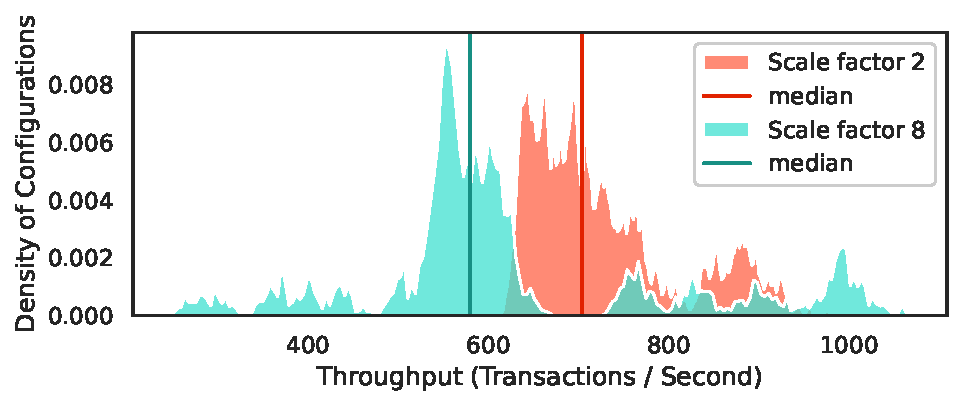
\includegraphics[width=\linewidth]{images/h2_intro.pdf}
	\caption{Throughput distribution of 1\,954 configurations of the database system \htwo, executing the \textsf{TPC-C} benchmark at two different scale factors.}
	\label{fig:h2_intro}
\end{figure}

Take as an example two performance throughput distributions across the configuration space of the database \htwo in Figure~\ref{fig:h2_intro}. Here,  the exact same configurations on two different parameterizations of the benchmark \textsf{TPC-C} have been measured In this scenario, the scale factor controls the modeled number of warehouses. While for most configurations, throughput decreases, for a larger benchmark, some configurations achieve even a higher throughput\footnote{A similar workload-specific performance distribution was  described by Pereira~et~ al. for the video encoder \xzwo~\cite{alves_sampling_2020}.}. That is, configuration-dependent performance can be highly sensitive to workload variation and the performance behavior under different workloads can change in unforeseeable ways. In turn, this can render performance models based on a single workload useless, unless configuration options’ sensitivity to workloads is accounted for.

To address this limitation, two different approaches have been pursued in the literature. 

The first approach relies on transfer learning techniques, where, given an existing performance model, in a separate step only the differences to a new environment are learned. A transfer function encodes which configuration options’ influence on performance is sensitive to workload variation. While transfer learning is an effective strategy that is not limited to varying workloads~\cite{jamshidi_learning_2018,jamishidi_transfer_2017,jamshidi_transfer_gp_2017,martin_transfer_2021,ding_bayesian_2020}, its main limitation is that the transfer function is specific to the differences between two environments.

In contrast to transfer learning, a second and more generalist approach is to consider the input fed to a software system as a further dimension for modeling performance. A workload is characterized by properties that---individually or in conjunction with software configuration options---influence performance. For such a strategy to work, one requires in-depth knowledge of the characteristics of a workload that influence performance. Let alone these characteristics can be mathematically modeled at all. This strategy has been effectively tested for a  variety of application-domains, such as program verification~\cite{koc_satune_2021} and high-performance computing codes~\cite{exastencils2014}. However, the added complexity comes at significant cost. 
Not only does it require substantially more measurements, we often lack knowledge of which performance-relevant characteristics best describe a workload (e.g., what makes a program hard to verify or optimize).

The existing body of research~\cite{dorn2020,siegmundPerformanceinfluenceModelsHighly2015,haDeepPerf2019,perfAL,guoVariabilityawarePerformancePrediction2013,sarkarCostEfficientSamplingPerformance,guo_2018_data,fourier_learning_2015,perLasso,chen_hinnperf_2022,chen_mmo_2021,nairUsingBadLearners2017,nairFlash18,ohFindingNearoptimalConfigurations2017} confirms the prevalence and importance of the workload influence on software systems. All these works are aware of the workload dimension as a factor of performance variation, yet little is known about the quality and driving factors of the \emph{interplay} between configuration options and workloads. Are workloads and configurations as factors influencing software performance orthogonal and can be treated independently or does their interplay give rise to intricate and inadvertent performance behavior?

We have conducted an empirical study that sheds light on whether and how choices of configuration and workload interact with regard to performance. 
Specifically, we analyzed 25\,258 configurations from nine configurable real-world software systems to obtain a broad picture of the interaction of configuration and workload when learning performance models and estimating a configuration's performance (i.e., response time). Aside from studying the sole effects of workload variation on performance behavior, we explore \textit{what} is driving the interaction between workload and configuration. To this end, we enrich performance observations with corresponding coverage data to understand workload variation with respect to executed code.


{
	\color{brown}
	We find that varying the workload can influence configuration-dependent software performance in different ways, including non-linear and non-monotonous effects. As a key take-away, we provide empirical evidence that single-workload approaches do not generalize across workload variations  and that even existing transfer learning techniques are too limited to address non-monotonous performance variations induced by qualitative workload changes. 
We demonstrate how code analyses such as coverage testing can outline a path to screen for workload-sensitive configuration options.
}

To summarize, we make the following contributions: 
\begin{compactitem}
	\item An empirical study of 25\,258 configurations from nine configurable software systems on whether and how interactions of workload and configuration affect software performance;
	{\color{black}
		\item A detailed analysis illustrating that (1) system-level performance, and (2) the performance influence of individual configuration options can be sensitive to workload variation and often exhibit a \textit{non-monotonous} relationship, caused by variation in the execution of option-specific  code;
		
		\item A critical reflection of the suitability of singular-workload models for predicting configuration-dependent performance and assumptions of state-of-the-art transfer learning approaches in this area;}
	
	\item {\color{brown}An archived repository~\cite{muhlbauer_workload_2023_companion} on \textit{zenodo.org} with supplementary material including performance and coverage measurements, configurations, and an interactive dashboard for data exploration to \textit{reproduce} all analyses and additional visualizations left out due to space limitations.}
\end{compactitem}

\section{Preliminaries and Related Work}
{
\color{brown}
Software performance emerges from a variety of factors including configuration, workload or hardware setup. In what follows, we revisit work that models the relationship between  such factors (individually or in combinations) and software performance.

}
\subsection{Performance Prediction Models}~\label{sec:perfmodels}
Configurable software systems are an umbrella term for any kind of software system that exhibits configuration options to customize their functionality. While the primary purpose of configuration options is to select and tune functionality, each configuration choice may also have implications on non-functional properties (execution time or memory usage)---be it intentional or not. 
Performance prediction models in this space approximate non-functional properties, such as execution time or memory usage, as a function of software configurations $c \in C$, formally $\Pi: C \rightarrow \mathbb{R}$. 


Such models do not rely on an understanding of the internals of a configurable software system, but are learned from a training set of configuration-specific performance observations. In this vein, finding configurations with optimal performance~\cite{chen_mmo_2021,nairUsingBadLearners2017,nairFlash18,ohFindingNearoptimalConfigurations2017} and estimating the performance for arbitrary configurations of the configuration space is an established line of research~\cite{dorn2020,siegmundPerformanceinfluenceModelsHighly2015,haDeepPerf2019,perfAL,guoVariabilityawarePerformancePrediction2013,sarkarCostEfficientSamplingPerformance,guo_2018_data,fourier_learning_2015,perLasso,chen_hinnperf_2022}.
Over the past years, several different learning and modeling techniques have shown to be effective to learn configuration-dependent software performance,  including probabilistic programming~\cite{dorn2020}, multiple linear regression~\cite{siegmundPerformanceinfluenceModelsHighly2015}, classification and regression trees~\cite{guoVariabilityawarePerformancePrediction2013,sarkarCostEfficientSamplingPerformance,guo_2018_data}, Fourier learning~\cite{fourier_learning_2015,perLasso}, and deep neural networks~\cite{haDeepPerf2019,perfAL,chen_hinnperf_2022}.
The set of configurations for training can be sampled from the configuration space using a variety of different sampling techniques~\cite{kaltenecker_interplay_2020,medeiros_comparison_2016}. All sampling strategies aim at yielding a representative sample, either by covering the main effects of configuration options and interactions among them~\cite{siegmundPredictingPerformanceAutomated2012}, or sampling uniformly from the configuration space~\cite{ohFindingNearoptimalConfigurations2017,kaltenecker_distance-based_2019}.
Most approaches share the perspective of treating a configurable software system as a black-box model at application-level granularity. Recent work has incorporated feature location techniques to guide sampling effort towards relevant configuration options~\cite{velez_2020_configcrusher_jase,velez_comprex_2021} or model non-functional properties at finer granularity~\cite{weber_white_2021,han_confprof_2021}.

{\color{black}
\subsection{Varying Workloads}\label{sec:varying_workloads}
%\subsubsection{Whats is a workload?}
When assessing the performance of a software system, we ask how well a certain \textit{operation} is executed, or, phrased differently, how well an \textit{input fed to the software system} is processed. 
{\color{brown}In the context of this study, we will refer to such inputs as \textit{workloads}.} By nature, the workload of a software system is application-specific, such as a series of queries and transactions fed to a database system or a set of raw image files processed by a video encoder. Workloads can often be distinguished by the characteristics they exhibit, such as the amount and type of data to be processed (text, binary data).

A useful workload for assessing performance should, in practice, closely resemble the real-world scenario that the system under test is deployed in. To achieve this, a well-defined and widely employed technique in performance engineering is workload characterization~\cite{ceesay2020,papadopoulos2021}. To select a representative workload, it is imperative to explore workload characteristics and validate a workload with real-world observations. This can be achieved by constructing workloads from usage patterns~\cite{calzarossa2016}, or by increasing the workload coverage by using a mix of different workloads rather than a single one~\cite{jiang2015survey}.

While workload characterization and benchmark construction is domain-specific, there are numerous examples of this task being driven by community efforts. For instance, the non-profit organizations Transaction Processing Performance Council (TPC) and Standard Performance Evaluation Corporation (SPEC) provide large bodies of benchmarks for data-centric applications or across different domains, respectively.
	
\subsection{Workloads and Performance Prediction} ~\label{sec:strategies}
Different approaches have been proposed to tackle the problem of workload sensitivity.

\paragraph{Workload-aware Performance Modeling}
\label{sec:workload-aware}
Extending on workload characterization (cf.~Section~\ref{sec:varying_workloads}), a strategy that embraces workload diversity is to incorporate workload characteristics into the problem space of a performance prediction model. Here, performance is modeled as a function of both the configuration options \textit{explicitly} exhibited by the software system as well as the workload characteristics, formally $\Pi: C \times W \rightarrow \mathbb{R}$.
The combined problem space enables learning performance models that generalize to workloads that exhibit characteristics denoted by $W$ since we can screen for performance-relevant combinations of options and workload characteristics. {\color{orange!50!red}This application-specific strategy has been successfully applied to domains such as program verification~\cite{koc_satune_2021}, algorithm selection~\cite{kotthoff_algorithm_selection_2016}, or the parametrization of the Java microbenchmark harness~\cite{samoaa_workload_2021}. In these instances, the characteristics (configurable aspects of a workload) are explicitly specified and do not require further characterization.}

 However, its main disadvantages are twofold: The combined problem space (configuration and workload dimension) requires substantially more observations to screen for identifying performance-relevant options, characteristics, and combinations thereof. In addition, previous work  found that  only few configuration options are sensitive to workload variation~\cite{jamishidi_transfer_2017}. That is, the problem of identifying meaningful, but sparse predictors is exacerbated since one must not only identify performance-relevant configuration options but also workload-sensitive ones. It is not possible to find such a characterization in every case. Even worse, a chosen characterization can be wrong and omit important factors or overestimate unimportant factors.
 
 {\color{red!50!orange} At large, the notion of the influence of workloads on configuration-dependent performance remains the exception in the literature: While a study related to ours explores and confirms the presence of interactions between the workload and configuration options, only few works even consider this dimension of the problem space~\cite{lesoil_2021}. }


\paragraph{Transfer Learning for Performance Models}\label{sec:transfer}
Another strategy builds on the fact that, across different workloads, only few configuration options are in fact workload sensitive~\cite{jamishidi_transfer_2017}. One first trains a model on a standard workload and, subsequently, adapts it to a different workload of choice. Contrary to a generalizable workload-aware model, transfer learning strategies focus on approximating a transfer function that, without characterizing the workload, encodes the information of which configuration options are sensitive to differences between a source and target pair of workloads. Training a workload-specific model and adapting it on demand provides an effective means to reuse performance models, which is not only limited to workloads~\cite{jamshidi_learning_2018, ding_bayesian_2020,valov_transferring_performance_2017,martin_transfer_2021}. The main shortcoming of transfer learning is that it does not generalize to arbitrary workloads, since a transfer function is tailored to a specific target workload. Basically, one trades off generalizability for measurement cost because learning a transfer function requires substantially fewer training samples.

While both directions (workload-aware performance modeling and transfer learning) are effective means to handle workload sensitivity, to the best of our knowledge, there is no \textit{systematic} assessment of the factors that drive the interaction between configuration options and workloads with regard to performance. Understanding scenarios that are associated with or even cause incongruent performance influences across workloads (1) help practitioners to employ established analysis techniques more effectively and (2) motivate researchers to devise analysis techniques dedicated to such scenarios.

\section{Study Design}~\label{sec:study}
In what follows, we describe our research questions and measurement setup. We make all performance measurement data, configurations, workloads, and learned performance models available on the paper's companion Web site~\cite{muhlbauer_workload_2023_companion}.

\subsection{Research Questions}
The first two research questions investigate the workload sensitivity of the studied software systems' performance behavior. We first take a look at the entire system~(\RQref{1}) with regard to a large set of configurations and, subsequently, to individual configuration options~(\RQref{2}). Furthermore, we explore possible driving factors and indicators for workload-specific performance variation of configuration options (\RQref{3}) {\color{brown} later on in Sec.~\ref{sec:new_section}}.

\subsubsection{Performance Variation Across Workloads}
Performance variation can arise from workload variation~\cite{benchmarking_book}. In a practical setting, the question arises whether, and if so, to what extent an existing workload-specific performance model is representative of the performance behavior of also other workloads. 
That is, can a model estimating the performance of different configurations be reused for the same software system but run with a different workload? 
Clearly, it depends. But, analyzing systematically on how the degree of similarity of workloads and corresponding performance behaviors varies across the configuration space provide insights to what extent the strategies of transfer performance models (outlined in Section~\ref{sec:strategies}) might be applicable.
To this end, we formulate the following research question: 

\RQ{1}{To what extent does \textit{performance behavior} vary across workloads and configurations?}
\subsubsection{Option Influence Across Workloads}
The global performance behavior emerges from the influences of several individual options and their interaction as well as the combined influence with the workload on performance. To understand which configuration options are driving performance variation, in general, and which are workload sensitive, in particular, we state the following research question:

\RQ{2}{To what extent do \textit{influences of individual configuration options} depend on the workload?}

\subsection{Experiment Setup}\label{sec:setup}
\subsubsection{Subject System Selection}
{\color{black}
We selected nine configurable software systems for our study. To ensure that our findings are not specific to one domain or ecosystem, we include a mix of Java and C/C++ systems from different application domains (cf. Table~\ref{tab:subject_systems}). In particular, we include systems studied in previous and related work~\cite{velez_2020_configcrusher_jase,weber_white_2021,alves_sampling_2020} and incorporate further ones with comparable size and configuration complexity (in terms of numbers of configurations and configuration options). All systems operate by processing a domain-specific workload fed to them. This study treats execution time as the key performance indicator with the exception of \htwo, where we report throughput.

\begin{table}
	\footnotesize
	\centering
	\caption{Subject System Characteristics}
	

\begin{tabular}{p{1.1cm}p{0.6cm}p{1.9cm}p{0.99cm}p{0.2cm}rrr}
	\toprule
	\textbf{System} & \textbf{Lang.} & \textbf{Domain} & \textbf{Version} & \textbf{\#\,O} & \textbf{\#\,C} & \textbf{\#\,W}  \\
	
	
	\midrule
	\jumper & Java & Audio Encoder & 1.0.4 & 16 & 4\,196 & 6   \\
	
	\kanzi &Java  & File Compressor & 1.9 & 24 & 4\,112 & 9 \\
	
	\dconvert & Java & Image Scaling & 1.0.0-$\alpha$7 & 18 & 6\,764 & 12  \\
	
	\htwo & Java & Database & 1.4.200 & 16 & 1\,954  & 8  \\
	
	\batik & Java & SVG Rasterizer & 1.14 & 10 & 1\,919 &  11  \\

	\midrule
	
	\xz & C/C++ & File Compressor & 5.2.0 & 33 & 1\,999 & 13  \\
	\lrzip & C/C++ & File Compressor & 0.651 & 11 & 190 & 13  \\
	%\rowcolor{red!10}\flac & C/C++ & Audio Encoder & 1.3.4 & -- & -- & --  \\
	%\rowcolor{red!10}\vpnine & C/C++ & Video Encoder & 1.1.0 & -- & -- & --  \\
	
	\xzwo & C/C++ & Video Encoder & baee400\ldots & 25 & 3\,113 & 9  \\
	\zdrei & C/C++ & SMT Solver & 4.8.14 & 12 & 1\,011 & 12  \\
	
	\bottomrule
	
\end{tabular}\\
{\centering\vspace{1mm}\textit{\#\,O: No. of options, \#\,C: No. of configurations, \#\,W: No of. workloads tested}}
	

	\label{tab:subject_systems}
\end{table}

\subsubsection{Workload Selection}
This study relies on a selection of workloads for each domain or software system. Ideally, each set of workloads is diverse enough to be representative of most possible use cases. We selected the workload sets in this spirit, but cannot always guarantee a measurable degree of diversity and representativeness prior to conducting the actual measurements. Basically, this it what motivates this study in the first place. Nevertheless, we discuss this aspect as a threat to validity in Sections~\ref{sec:threats}. Next, we outline the nine subject systems along with the workloads tested. 

For the \textit{audio encoder} \jumper, the measured task was to encode raw WAVE audio signals to MP3 (\jumper). We selected a number of different audio files from the Wikimedia Commons collection\footnote{Wikimedia Commons image collection: \url{https://commons.wikimedia.org/wiki/Category:Images}} and aimed at varying the file size/signal length, sampling rate, and number of channels. Both applications share all workloads.

For the \textit{video encoder} \xzwo, the measured task was to encode raw video frames (y4m format). We selected a number of files from the “derf collection”\footnote{``derf collection'' of the Xiph.org video test data:\url{https://media.xiph.org/video/derf/}}, a set of test media for a variety of use cases. The frame files vary in resolution (low/SD up to 4K) and file size. For files with 4K resolution, we limited our measurements to encoding a subset of consecutive frames.

For the \textit{file compression} tools \kanzi, \xz, and \lrzip, we used a variety of community compression benchmarks that represent different goals, including mixes of files of different types (text, binary, structured data etc.) or single-type files. We augmented this set of workloads with custom data, such as the Hubble Deepfield image and a binary of the Linux kernel. Beyond this set of workloads, for \xz and \lrzip, we added different parameterizations of the UIQ2 benchmark\footnote{Generic Compression Benchmark by Matt Mahoney: \url{http://mattmahoney.net/dc/uiq/}} to study the effect of varying file size. 

For the \textit{SMT solver} \zdrei, the measured task was to decide the satisfiability (find a solution or counter example) of a range of logical problems expressed in the SMT2 format. We selected the six longest-running problem instances from z3’s performance test suite and augmented it with additional instances from the SMT2-Lib repository\footnote{SMT competition 2017 benchmarks: \url{https://smt-comp.github.io/2017/benchmarks.html}}, to cover different types of logic and to increase diversity.

For the \textit{SVG rasterizer} \batik, the measured task was to transform a SVG vector graphic into a bitmap. We selected a number of resources from the Wikimedia Commons collection, primarily varying the file size. 

For the embedded \textit{database} \htwo, we used a selection of four benchmarks (SmallBank, TPC-H, YCSB, Voter) from \textsc{OLTPBench}~\cite{difallah_oltp_2013}, a load generator for databases. For each benchmark, we varied the scale factor, which controls the complexity (number of entities modeled) in each scenario.

For the \textit{image scaler} \dconvert, the measured task was to transform resources (image files, Photoshop sketches) at different scales (useful for Android development). We selected files that reflect \dconvert's documented input formats (JPEG, PNG, PSD, and SVG) and vary in file size.
}

\subsubsection{Configuration Sampling}\label{sec:sampling}
For each subject system, we sampled a set of configurations. As exhaustive coverage of the configuration space is infeasible due to combinatorial explosion~\cite{henardCombining2015}, for binary configuration options, we combine several coverage-based sampling strategies and uniform random sampling into an \emph{ensemble} approach: 
We employ option-wise and negative option-wise sampling~\cite{siegmundPerformanceinfluenceModelsHighly2015}, where each option is enabled once (i.e., in, at least, one configuration), or all except one, respectively. In addition, we use pairwise sampling, where two-way combinations of configuration options are systematically selected. Interactions of higher degree could be found accordingly, however, full interaction coverage is computationally prohibitively expensive~\cite{henardCombining2015}. 
Last, we augment our sample set with a random sample that is, at least, the size of the coverage-based sample. To achieve a nearly uniform random sample, we used \emph{distance-based sampling}~\cite{kaltenecker_distance-based_2019}. If a software system exhibited numeric configuration options, we varied them across, at least, two levels to measure their effect.

\subsubsection{Coverage Profiling}\label{sec:profiling}
To assess what lines of code are executed for each combination of workload and software configuration, we used two separate approaches for Java and C/C++. For Java, we used the on-the-fly profiler \textsc{Jacoco}\footnote{\textsc{Jacoco}: \url{https://www.jacoco.org/jacoco/trunk/doc/}}, which intercepts byte code running on the JVM at run-time. For C/C++, we added instrumentation code to the software systems using \textsc{Clang/LLVM}\footnote{\textsc{LLVM}: \url{https://clang.llvm.org/docs/SourceBasedCodeCoverage.html}} to collect coverage information. We split the performance measurement and coverage analysis runs to  avoid distortion from the profiling overhead.
	
\subsubsection{Measurements}\label{sec:measurement_setup}
All experiments were conducted on three different compute clusters, where all machines within a compute cluster had the identical hardware setup: Cluster A with an Intel Xeon E5-2630v4 CPU (2.2\,GHz) and 256\,GB of RAM, cluster B  with an Intel Core i7-8559U CPU (2.7\,GHz) and 32\,GB of RAM, and cluster C with an Intel Core i5-8259U (2.3\,GHz) and 32\,GB of RAM. All clusters ran a headless Debian 10 installation (kernel 4.19.0-17 for cluster A and 4.19.0-14 for clusters B and C). To minimize measurement noise, we used a controlled environment, where no additional user processes were running in the background, and no other than necessary packages were installed. 
We ran each subject system \textit{exclusively} on a single cluster: \htwo on cluster A; \dconvert and \batik on cluster B; the remaining systems on cluster C.

{\color{brown}We collect performance cata using the tools \textsc{GNU time} (execution time) and \textsc{OLTPBench} (throughput).} For all data points, we report the median {\color{brown}performance} across five repetitions (except for \htwo), which has shown to be a good trade-off between variance and measurement effort~\cite{molyneauxArtApplicationPerformance2015}. 
{\color{brown}Across these repetitions, most configurations exhibit only little variation (e.g., only a few seconds for whole-system benchmarks which run for several minutes): the ratio of configurations with a coefficient of variation (standard deviation divided by the mean) of less than 10\,\% ranges from 91\,\% (\lrzip) for \lrzip to 99\,\% (\xzwo).}
For \htwo, we omitted the repetitions as, in a pre-study, running on the identical cluster setup, we found that across all benchmarks the coefficient of variation of the throughput was consistently below 5\,\%.

\section{Study Results}~\label{sec:results}
In this section, we present the results of our empirical study with regard to variation of system-level performance distributions (\RQref{1}) and the performance influence of individual configuration options (\RQref{2}) as well as the relationship between configuration-specific code-coverage and workload variation (\RQref{3}). 

\subsection{Comparing Performance Distributions ($\text{RQ}_\text{1}$)}\label{sec:rq1}
\subsubsection{Operationalization}
We answer \RQref{1} by pairwisely comparing the performance distributions from different workloads (cf. the comparison in Figure~\ref{fig:h2_intro}) and by determining whether any two distributions are similar or, if not, can be transformed into each other: For the former case, we tested all combinbations of workload-specific performance observations with the Wilcoxon signed-rank test\footnote{We use non-parametric methods since performance-distributions are often long-tailed and multi-modal~\cite{curtsinger_stabilizer_2013,maricq2018taming} and, thus, fail to meet requirements for parametric methods.}~\cite{lovric_international_2010}. For all combinations, we rejected the null hypothesis $H_0$ at $\alpha=0.95$. To account for overpowering due to high and different sample sizes (cf.~Table~\ref{tab:subject_systems}), we further checked effect sizes to weed out negligible effects. Following the interpretation guidelines from Romano et al.~\cite{romano2006exploring}, for no combination, Cliff's~$\delta$~\cite{Cliff1993DominanceSO} exceeded a threshold effect size of $\vert\delta > 0.147\vert$.
For the latter case, we are specifically interested in what \textit{type} of transformation is necessary as this determines, \textit{how} complex a workload interacts with configuration options. Specifically, we categorize each pair of workloads with respect to the following aspects: 

\begin{compactenum}

	\item \textit{Linear Correlation}: To test whether both performance distributions are shifted by a constant value or scaled by a constant factor, we compute for each pair of distributions Pearson's correlation coefficient $r$. To discard the sign of relationship, we use the absolute value and a threshold of $\vert r\vert >0.6$ to indicate a linear relationship.
	
	\item \textit{Monotone Correlation}: We test whether there exists a monotonous relationship between the two performance distributions. We use Kendall's rank correlation coefficient $\tau$~\cite{kendall1938new} and a threshold of  $\vert\tau\vert > 0.6$ for a monotonous relationship.
\end{compactenum}
{\color{black}Based on these two correlation measures, we composed three categories that each pair of performance distributions can be categorized into.
If both distributions exhibit a strong linear relationship, we classify them as linearly transformable (\textit{\colorbox{lt-color!60}{LT}}). If we observe a strong monotonous, but not a linear relationship, we classify such pairs as exclusively monotonously transformable into a separate category (\textit{\colorbox{xmt-color!60}{XMT}}). Last, we have the pairs with a non-monotonous relationship  (\textit{\colorbox{nmt-color!60}{NMT}}). 
We summarize the category criteria as well as the category counts in Table~\ref{tab:categorization}. 

\begin{table}
	\footnotesize
	\caption{Three disjoint categories and criteria of relationships between pairs of workload-specific performance distributions.}
	\centering
\begin{tabular}{lp{4.1cm}p{2.8cm}}	
	\toprule
	 \textbf{} & \textbf{Category} & \textbf{Criteria}\\
	 \midrule
	 %\cellcolor{cs-color}\textit{SD} & {Statistically similar distributions} & {$H_0$ not rejected} and $\delta > 0.147$ \\
	 \rowcolor{lt-color!40!white}\cellcolor{lt-color}\textit{\textbf{LT}} & {Linear transformation} & $r^* \geq 0.6$ \\
	\rowcolor{xmt-color!40!white}\cellcolor{xmt-color}\textit{\textbf{XMT}} & {Monotonous transformation} & $r^* < 0.6 $ and $ \tau^* \geq 0.6$ \\
	\rowcolor{nmt-color!40!white}\cellcolor{nmt-color}\textit{\textbf{NMT}} & {Non-monotonous transformation}  & (otherwise) \\%$p < 0.05$ and $\tau < 0.6$ \\
	\bottomrule
\end{tabular}
\label{tab:categorization}
\end{table}

\begin{table}
	\footnotesize
	\centering
	\caption{Frequency of each category (cf. Table~\ref{tab:categorization}) for each software system studied and pairs of workloads.}
\begin{tabular}{p{1.1cm}rrrrrrr}	
	\toprule
	\textbf{System} & \textbf{$\Sigma_\text{pairs}$} & \multicolumn{2}{c}{\textbf{\cellcolor{lt-color}\textit{LT}}} & \multicolumn{2}{c}{\textbf{\cellcolor{xmt-color}\textit{XMT}}} & \multicolumn{2}{c}{\textbf{\cellcolor{nmt-color}\textit{NMT}}}\\
	  & & \textit{abs} &\textit{rel} & \textit{abs} & \textit{rel}& \textit{abs} & \textit{rel}\\
	\midrule
	
	\jumper & \textit{15} &
	%0 & 0\,\% & 
	\cellcolor{lt-color!100!white}15 & \cellcolor{lt-color!100!white}100.0\,\% & 
	0 & 0\,\% & 
	0 & 0\,\%\\
	
	\kanzi & \textit{36} &
	%0 & 0\,\% & 
	\cellcolor{lt-color!78!white}28 & \cellcolor{lt-color!78!white}77.8\,\% & 
	\cellcolor{xmt-color!11!white}	4& \cellcolor{xmt-color!11!white}11.1\,\% & 
	\cellcolor{nmt-color!11!white}4 & \cellcolor{nmt-color!11!white}11.1\,\%\\
	
	\dconvert & \textit{66} &
	%0 & 0\,\% & 
	\cellcolor{lt-color!43!white}29 & \cellcolor{lt-color!43!white}43.9\,\% & 
	0 & 0\,\% & 
	\cellcolor{nmt-color!56!white}37 & \cellcolor{nmt-color!56!white}56.1\,\%\\
	
	\htwo & \textit{28} &
	%0& 0\,\% & 
	\cellcolor{lt-color!47!white}13 & \cellcolor{lt-color!47!white}46.4\,\% & 
	0 & 0\,\% & 
	\cellcolor{nmt-color!53!white}15 & \cellcolor{nmt-color!53!white}53.6\,\%\\
	
	\batik & \textit{55} &
	%0 & 0\,\% & 
	\cellcolor{lt-color!50!white}28 & \cellcolor{lt-color!50!white}50.9\,\% & 
	\cellcolor{xmt-color!14!white}8 & \cellcolor{xmt-color!14!white}14.6\,\% & 
	\cellcolor{nmt-color!34!white}19 & \cellcolor{nmt-color!34!white}34.6\,\%\\
	
	\midrule
	
		\xz & \textit{78} &
	%0 & 0\,\% & 
	\cellcolor{lt-color!83!white}65 & \cellcolor{lt-color!83!white}83.3\,\% & 
	\cellcolor{xmt-color!1!white}1 & \cellcolor{xmt-color!1!white}1.3\,\% & 
	\cellcolor{nmt-color!15!white}12 & \cellcolor{nmt-color!16!white}15.4\,\%\\
	
		\lrzip & \textit{78} &
	%0 & 0\,\% & 
	\cellcolor{lt-color!73!white}57 & \cellcolor{lt-color!73!white}73.0\,\% & 
	\cellcolor{xmt-color!16!white}13 & \cellcolor{xmt-color!16!white}16.7\,\% & 
	\cellcolor{nmt-color!10!white}8 & \cellcolor{nmt-color!10!white}10.3\,\%\\
	
	\xzwo & \textit{36} &
	%0 & 0\,\% & 
	\cellcolor{lt-color!100!white}36 & \cellcolor{lt-color!100!white}100\,\% & 
	0 & 0\,\% & 
	0 & 0\,\%\\
	
	\zdrei & \textit{66} &
	%0 & 0\,\% & 
	\cellcolor{lt-color!15!white}10 & \cellcolor{lt-color!15!white}15.2\,\% & 
	\cellcolor{xmt-color!2!white}1 & \cellcolor{xmt-color!2!white}1.5\,\% & 
	\cellcolor{nmt-color!83!white}55 & \cellcolor{nmt-color!83!white}83.3\,\%\\
	
	\bottomrule
	\end{tabular}
	\label{tab:categorization_counts}
\end{table}

\subsubsection{Results}
{\color{black}
We depict the results of our classification in Table~\ref{tab:categorization_counts}. The observed range of relationships across the nine software systems exhibit no type that prevails across all software systems. 
All software systems, at least, in part, exhibit performance distributions that can be transformed into one another using a linear transformation (\textit{\colorbox{lt-color!60}{LT}}), such as shifting by a constant value or scaling by a constant factor. In particular, for \jumper and \xzwo, we observe solely such behavior. The presence of linear transformations corresponds to experimental insights from Jamshidi et al., who encoded differences between performance distributions using linear functions~\cite{jamishidi_transfer_2017}.

Exclusively monotone transformations (\textit{\colorbox{xmt-color!60}{XMT}}) are the exception and are exhibited only by five out of the nine systems (\kanzi, \batik, \xz, \lrzip, \zdrei), twice with only one workload pair each (\xz and \zdrei).  
For all, except two systems (\jumper and \xzwo), we observe non-monotonous relationships (\textit{\colorbox{nmt-color!60}{NMT}}) with different prevalence.  For three systems (\dconvert, \htwo, and \zdrei), the majority of transformations required is non-monotonous; for the other four systems (\kanzi, \batik, \xz, \lrzip), more than 10\,\% of workload pairs fall into this category.
\greybox{\textbf{Summary} (\RQref{1}): Varying the workload causes a substantial amount of variation among performance distributions. Across workloads, we observed \textit{mostly linear} (for six of the nine subject systems), but to a large extent, also \textit{non-monotonous} relationships (for three of the nine subject systems).
}

\subsection{Workload Sensitivity of Individual Options ($\text{RQ}_\text{2}$)}\label{sec:rq2}
\subsubsection{Operationalization}
To address \RQref{2}, we need to determine the configuration options’ influence on performance and assess their variation across workloads. 
\paragraph*{Explanatory Model}
To obtain accurate and interpretable performance influences per option, we learn an explanatory performance model based on the entire sample set using multiple linear regression~\cite{dorn2020,siegmundPerformanceinfluenceModelsHighly2015,perLasso}. Here, each variable in the linear model corresponds to an option, and each coefficient represents the corresponding option's influence on performance. 
We limit the set of independent variables to individual options rather than including higher-order interactions to be consistent with the feature location used for \RQref{3}, where we determine option-specific, yet not interaction-specific code segments.
\paragraph*{Standardization}
To facilitate the comparison of regression coefficients across workloads, we follow common practice in machine learning and standardize our dependent variable by subtracting the population’s mean performance and divide the result by the respective standard deviation. Henceforth, we refer to these standardized regression coefficients as \textit{relative performance influences}. A beneficial side effect of standardization is that the observed variation of regression coefficients for each configuration option cannot be attributed to shifting or scaling effects (\colorbox{lt-color!60}{\textit{LT}}). This way, we can pin down  the non-linear or explicitly non-monotonous effect that workloads may exercise on performance.
\paragraph*{Handling Multicollinearity} Multicollinearity is a standard problem in statistics and emerges when features are correlated~\cite{Daoud_2017}. This can, for instance, arise from groups of mutually exclusive configuration options and result in distorted regression coefficients~\cite{dorn2020}. Although the model's prediction accuracy remains unaffected, we cannot trust and easily interpret the calculated coefficients. To mitigate this problem and, in particular, to ensure that the obtained performance influences remain interpretable, we follow best practices and remove specific configuration options from the sample that cause multicollinearity~\cite{dorn2020}. For the training step, we exclude all mandatory configuration options since these, by definition, cannot contribute to performance variation. In addition, for each group of mutually exclusive configuration options, we discard one group member when learning a model. These measures reduced multicollinearity to a negligble degree~\cite{o2007caution}. Specifically, after these corrections, we observed no configuration options exceeding a variance inflation factor (indicating multicollinearity) of 5.


\subsubsection{Results}\label{sec:results2}

\begin{figure*}
	\centering
	\begin{subfigure}{0.29\linewidth}
		\centering
		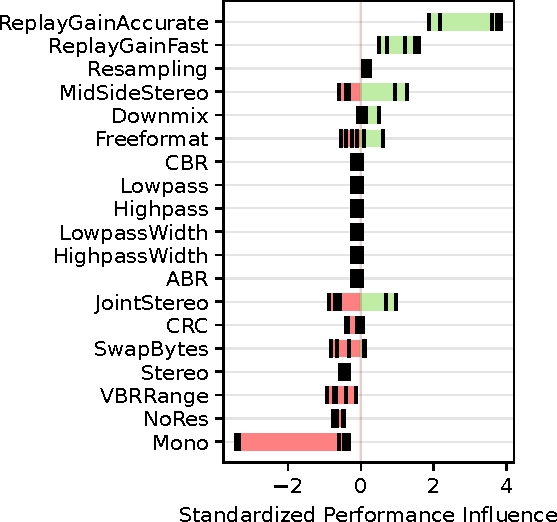
\includegraphics[width=\linewidth]{images/jump3r.pdf}
		\caption{\jumper}
		\label{fig:overview_jump3r}
	\end{subfigure}
	\begin{subfigure}{0.29\linewidth}
		\centering
		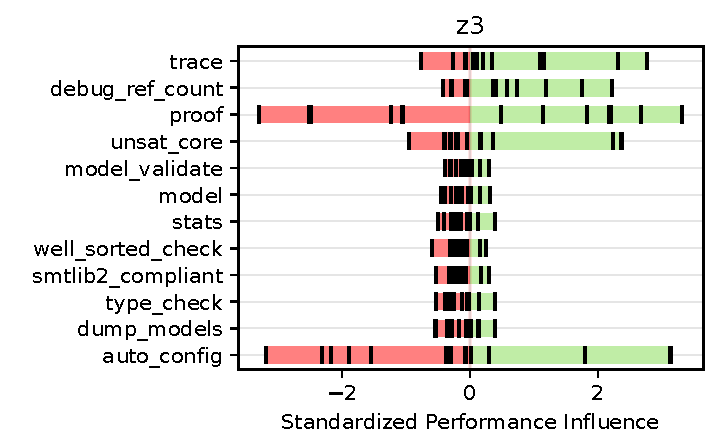
\includegraphics[width=\linewidth]{images/z3.pdf}
		\caption{\zdrei}
		\label{fig:overview_z3}
	\end{subfigure}
	\begin{subfigure}{0.4\linewidth}
		\centering
		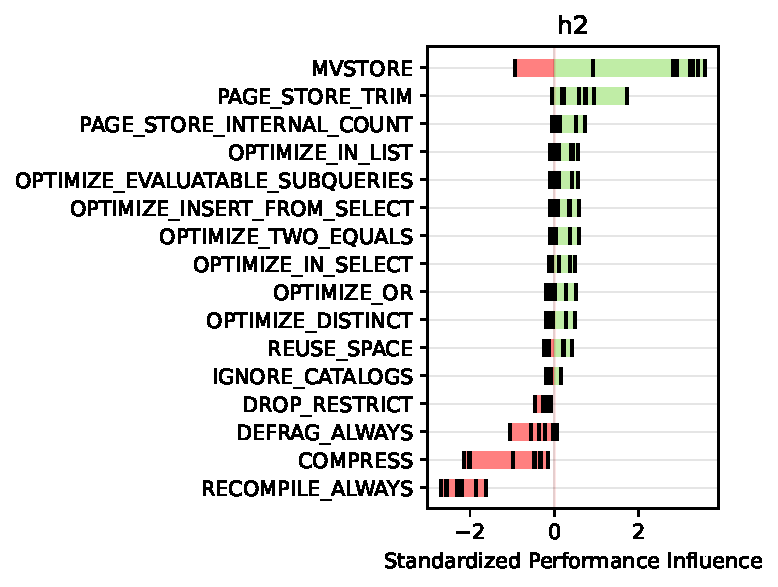
\includegraphics[width=\linewidth]{images/h2.pdf}
		\caption{\htwo}
		\label{fig:overview_h2}
	\end{subfigure}
	
	\caption{Distribution of configuration options' performance influences under different workloads for \jumper, \zdrei, and \htwo. Each vertical bar depicts the performance influence under a specific workload. The observed ranges of positive and negative influences are highlighted in green and red, respectively.}
	\label{fig:three_systems}
\end{figure*}
	
Our results show a wide variety of workload sensitivity. Due to the size of our empirical study and space limitations, we selected three configuration options that showcase different characteristic traits of observed workload sensitivity. The exhaustive analysis for all configuration options is illustrated in terms of an interactive dashboard provided as supplementary material. We strongly invite the interested reader to use this interactive dashboard to explore all distributions and results obtained in this study.

{In Figure~\ref{fig:three_systems}, we show the distribution of configuration options' performance influences for three of the nine software systems (\jumper, \zdrei, and \htwo). {\color{black}Each vertical bar depicts the relative performance influence under a specific workload, the colored ranges depict positive (green) and negative (red) performance influences. The following patterns refer to one row in Figures~\ref{fig:overview_jump3r}, \ref{fig:overview_z3}, and \ref{fig:overview_h2} (configuration option) for one subject system each.}

\paragraph{Conditional Influence}\label{sec:conditional_influence} For some configuration options, we observe that they affect performance only under specific workloads and remain non-influential otherwise. An example of such conditional influence is the configuration option \textsf{Mono} for the MP3 encoder \jumper. We illustrate the performance influence of this option across six workloads presented as bar plots in Figure~\ref{fig:mono_jump3r}. Selecting this option reduced the execution time substantially for two workloads, whereas, for the other workloads, the effect was far smaller.

According to the documentation of \jumper\footnote{\jumper: \url{https://github.com/Sciss/jump3r/blob/master/README.md}}, selecting this option for stereo files (i.e., audio files with two channels) results in averaging them into one channel. Indeed, the two workloads described above are the only ones that exhibit two audio channels in this selection. Hence, this example illustrates how a workload  characteristic can condition the performance influence of a configuration option. 

\paragraph{High Spread} Another pattern we found is that the performance influence of most (relevant) configuration options exhibits a large spread. For example, option \textsf{proof} of the SMT solver \zdrei can both increase or decrease the execution time as shown in Figure~\ref{fig:proof_z3}. Compared to the example above, we cannot attribute this variation to an apparent workload characteristic.
The global parameter \textsf{proof} enables tracking information, which is used for proof generation in case a problem instance is unsatisfiable. Each workload in our selection contains multiple problem instances to decide satisfiability for. We conjecture that the ratio of satisfiable to unsatisfiable instances likely accounts for this high variation. From the user's perspective, any input to the solver is opaque in that satisfiability as a workload characteristic cannot be determined practically without a solver. 
\paragraph{Scaling Anomaly} The anomaly pattern is shown for the configuration option \textsf{MVSTORE} of the database system \htwo in Figure~\ref{fig:mvstore_h2} (left). The option controls which storage engine, either the newer multi-version store or the legacy page store, is used. We observe that selecting the newer multi-version store increases the measured throughput for all but one benchmark scenario. When tested with the Yahoo! Cloud Serving Benchmark (YCSB) with two different scale factors (that control the workload complexity; expressed as number of rows), we found that the less complex parameterization (\textsf{ycsb-600}) results in a lower throughput. This is in stark contrast to the expectation that a more complex workload would show lower throughput. While it is possible that some optimizations of the multi-version store are effective only under higher load, this example demonstrates that performance influence is not guaranteed to scale with the workload as expected. 
\greybox{\textbf{Summary} (\RQref{2}): Workloads can affect performance influences of configuration options in various ways (e.g., conditioning influence, introducing variance, having outliers). We can correlate some variation of performance influences with workload characteristics, yet identifying relevant workload characteristics is highly domain-specific and cannot be considered trivial. 
}

}

\begin{figure}
	\centering
	\begin{subfigure}{\linewidth}
		\centering
		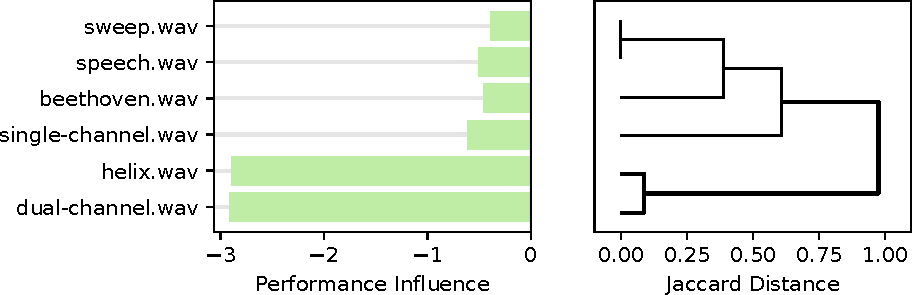
\includegraphics[width=0.96\linewidth]{images/Mono.pdf}
		\caption{Performance influence (left) and option-code coverage clustering for option \textsf{Mono} (\jumper).}
		\label{fig:mono_jump3r}
	\end{subfigure}
	
	\begin{subfigure}{\linewidth}
		\centering
		\vspace{2em}
		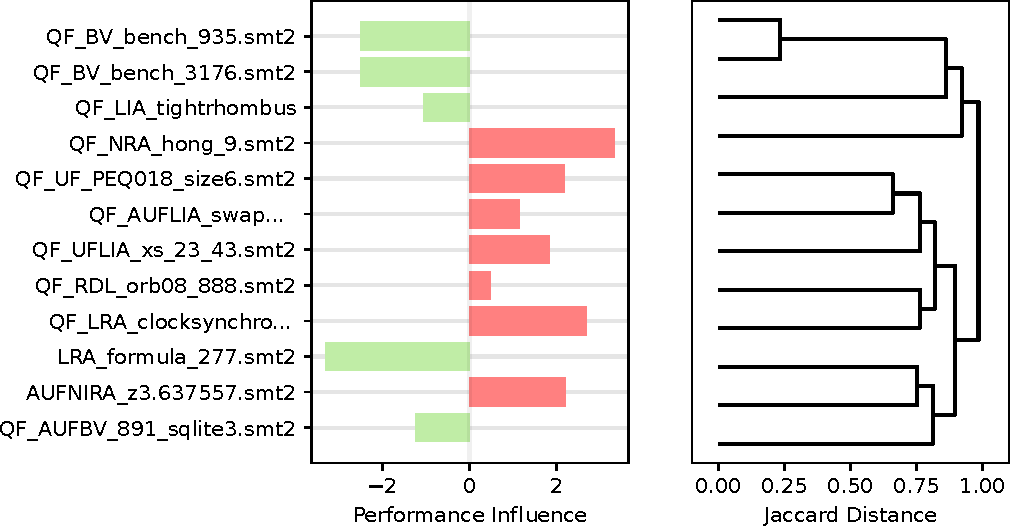
\includegraphics[width=0.96\linewidth]{images/proof.pdf}
		\caption{Performance influence (left) and option-code coverage clustering for option \textsf{proof} (\zdrei).}
		\label{fig:proof_z3}
	\end{subfigure}

	\begin{subfigure}{\linewidth}
		\centering
		\vspace{2em}
		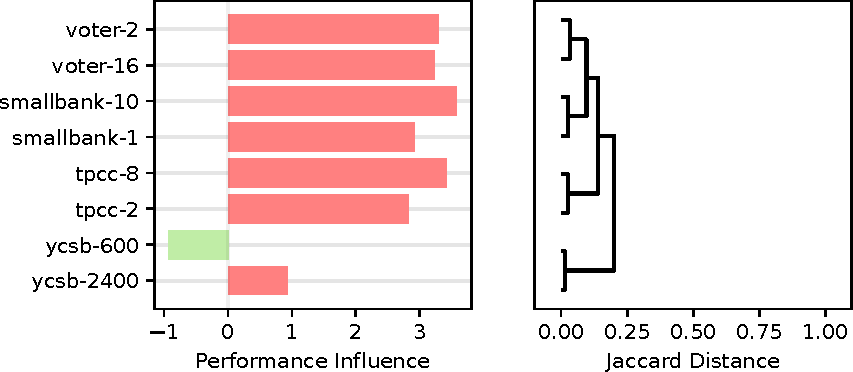
\includegraphics[width=0.96\linewidth]{images/MVSTORE.pdf}
		\caption{Performance influence (left) and option-code coverage clustering for option \textsf{MVSTORE} (\htwo).}
		\label{fig:mvstore_h2}
	\end{subfigure}
\caption{Workload-dependent performance influences of configuration options \textsf{Mono} (\jumper), \textsf{proof} (\zdrei), and \textsf{MVSTORE} (\htwo) (left) and option-code coverage clusterings for the the configuration options (right).}
\end{figure}

\label{sec:rq3}\label{sec:categories}
\color{orange}
\section{Exploring Causes of Workload Sensitivity}\label{sec:new_section}
The results for the first two research questions demonstrate configuration options’ sensitivity to the workload due to non-monotonous interactions and are consistent with the findings of a related study~\cite{lesoil_2021}. Before we discuss implications for performance modeling in the next section, we aim at understanding the underlying factors that drive workload sensitivity.

We hypothesize that executions under different workloads also exhibit variation with respect to what code sections are executed (and which are not) and how this code is used (e.g., number of method invocations or loop passes). Differences in performance influences of individual methods may stem from differences in program execution. Depending on whether an option is active or what value it has been set to, we may visit different code sections of the program or change their intensity. We are interested in how far one could infer or even explain performance variations just based on standard code-coverage analyses. That is, we ask whether we can explain the workload sensitivity of configuration options influences at the code level:

\RQ{3}{Does the variation of performance influence of configuration options across workloads correlate with differences in the respective execution footprint?}

Exploiting a potential the relationship between workload sensitivity of configuration options and differences in software execution could be practical. Instead of testing various combinations of configurations and workloads, code analysis can serve as a cost-effective way to detect workload sensitivity by identifying workload-specific differences in program execution.

%\section{Relationship between Configuration-Specific Code Coverage and Workload Variation ($\text{RQ}_\text{3}$)}
\subsection{Operationalization}To explore whether and to what extent variations in the execution paths (that stem from the interplay of the given workload and configuration) correlate with performance variations, we employ an analysis based on code coverage information~(cf.~Sec.~\ref{sec:profiling}). That is, we augment our performance observations with code coverage information to assess differences in the execution under different workloads. Specifically, we are interested in code sections that implement option-specific functionality. From comparing the coverage information of option-specific code, we can formulate different hypothetical scenarios explaining workload sensitivity. 

\textit{First}, if we observe that the  coverage of option-specific code is conditioned by the presence of some workload characteristic, we expect that such an option is only influential under corresponding workloads. This scenario enables us (to some extent) to use code coverage as a cheap-to-compute proxy for estimating the representativeness of a workload and, by extension, resulting performance models: For options that are known to condition code sections, we can maximize option-code coverage to elicit all option-specific behavior and, thus, performance influence. For instance, a database system could cache a specific view only if a minimum number of queries are executed. Here, the effect of any caching option would be conditioned by the workload-specific number of transactions.

\textit{Second}, if we observe performance variation across workloads in spite of similar or identical option-specific code coverage, we draw a different picture. In this case, we cannot attribute performance variation to code coverage, yet have to consider differences in the workloads’ characteristics as potential cause: The presence of a workload characteristic may influence not  \emph{what} code sections are executed, but \emph{how} code sections are executed. For instance, in a simple case, a software system’s performance may scale linearly with the workload size. In a more complex case, the presence of a characteristic may determine how frequently an operation is repeated, as is the case for a table merge operation in a database system. Here, we would not elicit the worst-case performance if a previous transaction has sorted the data (e.g., by building an index).
\color{black}

\subsubsection{Locating Configuration-Dependent Code}
To reason about option-specific code, we require a mapping of configuration options to code. 
The problem of determining which code section implements which functionality in a software system is known as \emph{feature location}~\cite{rubin_feature_2013}. 
While there is a number of approaches based on static~\cite{velez_2020_configcrusher_jase,lillack_2018_lotrack_tse,luo_2019_cova} and dynamic taint analysis~\cite{bell_phosphor_2014,velez_comprex_2021,splat_kim_2013}, we employ a more light-weight,  but also less precise approach that uses code coverage information, such as execution traces.
The rationale is that, by exercising feature code, for instance, by enabling configuration options or running corresponding tests, its location can be inferred from differences in code coverage. 
Applications of such an approach have been studied not only for feature location~\cite{wong_integrated_2005,sulir_annotation_2015,michelon_spectrum_2021,perez_framing_2016}, but root in work on program comprehension~\cite{wilde_early_1996,wilde_reconnaissance_1995,sherwood_reducing_nodate,perez_diagnosis_2014,castro_pangolin_2019} and fault localization~\cite{agrawal_fault_1995,wong_faultloc_2016}. 


Specifically, we follow  a strategy akin to  \textit{spectrum-based feature location}~\cite{michelon_spectrum_2021}:
We commence with obtaining a baseline of all code that can be associated with a configuration option in the scope of our workload selection. Since we are looking for workload-specific differences in option-code coverage, the expressiveness of such a baseline depends on the diversity of the workloads in question. To infer option-specific code, we split our configuration sample (cf. Section~\ref{sec:sampling}) into two disjoint sets $c_o$ and $c_{\neg o}$ such that option $o$ is selected only in $c_o$ and not in $c_{\neg_o}$. Next, we select from our code coverage logs the corresponding covered lines of code, $S_o$ and $S_{\neg o}$.  The rationale is that all shared lines between both sets are not affected by the selection of an option $o$. Thus, we compute the \textit{symmetric set difference} $\mathbb{S}_o = S_o~\Delta~S_{\neg o}$ to approximate option-specific or, at least, option-related code sections. To finally obtain code sections that are option-specific under a specific workload $w$, we repeat the steps above. Here, we consider only execution logs under workload $w$ ($S_{o, w}$ and $S_{\neg o, w}$) and compute the symmetric set difference $\mathbb{S}_{o,w}=S_{o,w}~\Delta~S_{\neg o, w}.$


\subsubsection{Comparing Execution Traces}
From (a) the information about which code sections are specific to a configuration option and (b) how much of these sections is actually covered under different workloads, we can compare the workload-specific execution traces for each option. By comparing the sets $\mathbb{S}_{o, v}$ and $\mathbb{S}_{o, w}$ for any two workloads $v$ and $w$, we can estimate the similarity between the option-code coverage via the Jaccard set similarity index. A Jaccard similarity of zero implies that there is no overlap in the code lines covered under each workload, whereas a Jaccard similarity of 1 implies that the exact same code was covered. Based on this pairwise similarity metric $sim_o(v, w)$, we can compute a corresponding distance metric $d_o(v, w) = 1 - sim(v, w)$ and cluster all workload-specific execution profiles. 
We use agglomerative hierarchical clustering with full linkage to construct dendrograms. In this bottom-up approach, we iteratively add execution footprints to clusters and merge sub clusters into larger ones depending on their Jaccard similarity  to each other. 

\subsection{Results}\label{sec:results3}
We report our findings for the relationship between execution footprints and performance influences for the same configuration options presented for \RQref{2}, since these illustrate likely causes of workload sensitivity and the limitations of solely relying on code coverage. The dashboard on the supplementary Web site provides diagrams and inferred feature code for all configuration options. The dendrograms next to the visualizations of performance influences in Figures \ref{fig:mono_jump3r}, \ref{fig:mvstore_h2}, and \ref{fig:proof_z3}, respectively, illustrate how similar the covered lines of option-specific code under each workload are. 
The dendrograms depict the Jaccard similarity clustering, where the split points indicate what Jaccard distance individual sets of lines or subclusters exhibit. The further to the left the point is, the more similar are the components.

We  observe that, in many cases, where  a configuration option is ``conditionally influential''~(cf.~Section~\ref{sec:conditional_influence}), the respective option-specific code under the interacting workloads fall into a cluster, as with the option-specific code for \textsf{Mono} in Figure~\ref{fig:mono_jump3r}. In this particular example, the dendrogram can be somewhat misleading as the number of common lines of code between workloads helix and dual-channel is far greater than between the other four workloads. Hence, differences in the coverage of option-specific code can account for, at least, some workload sensitivity.


The other two examples, the configuration options \textsf{proof} (\zdrei) and \textsf{MVSTORE} (\htwo), provide a different picture. Akin to the variation of performance influence of \textsf{proof}, the clustering for this configuration option (cf.~Figure~\ref{fig:mvstore_h2}) shows that some clusters are disjoint, and, thus, the option-specific code is highly fragmented depending on the workload. 

In the same vein, for \textsf{MVSTORE}, we see that the option-specific code is highly fragmented, yet all four benchmarks constitute clusters of high internal similarity. In the context of the observed variation of performance influences for the Yahoo! Cloud Serving Benchmark (YCSB), we see that even very high similarity in the covered code can virtually either improve or deteriorate performance.

For cases where we did not detect any differences in code coverage despite substantial differences in an option's performance influence across workloads, our results suggest that the way \emph{how} code was executed (i.e., how frequently methods or loops are executed) is shaping performance.

\greybox{\textbf{Summary} (\RQref{3}):  Varying the workload can condition the execution of option-specific code coverage and cause performance differences. However, there is no single driving cause of variation: Code utilization depending on workload characteristics is a likely further cause	accounting for the majority of variation in the performance influence of an option.
}
\color{black}
\section{Discussion}
Our results paint a clear picture of workload-induced performance variations of individual options. This sheds light on the extent of representativeness of singular-workload performance models. But, this is not the end of the story: We saw distinct patterns of complex variations that challenge transfer-learning approaches, which set out to overcome the workload specificity of models. Next, we discuss these points in more detail.


\subsection{Workload Sensitivity and Singular-Workload Approaches}
The observed workload sensitivity of configuration options exhibits a wide range of characteristics. While a large portion of options scales proportionally with workload complexity or remains unaffected by workload variation, the performance influences of several configuration options are sensitive to the workload.  So far, the existing body of work on modeling~\cite{dorn2020,siegmundPerformanceinfluenceModelsHighly2015,haDeepPerf2019,perfAL,guoVariabilityawarePerformancePrediction2013,sarkarCostEfficientSamplingPerformance,guo_2018_data,fourier_learning_2015,perLasso} and optimizing~\cite{chen_mmo_2021,nairUsingBadLearners2017,nairFlash18,ohFindingNearoptimalConfigurations2017} configuration-specific performance largely neglects the impact of workload variation at the cost of generalizability. 
Our findings from \RQref{2} demonstrate that individual configuration options becoming influential under specific workloads or shifting their influence from beneficial to detrimental (or vice versa) are not uncommon, which can distort performance estimations.

Beyond performance estimation, using performance models as surrogates for finding configurations with optimal performance properties is not without risk. For instance, there are several approaches utilizing the rank or importance of options~\cite{nairUsingBadLearners2017,ohFindingNearoptimalConfigurations2017}. Given the observed workload sensitivity, such rankings remain susceptible to the choice of workload.
\greybox{\textbf{Insight:} Workload sensitivity challenges the robustness and generalizability of singular-workload performance models, yet is neglected in state-of-the-art approaches. Even more, robust techniques using only rankings or relative importance of options are inapplicable for certain workload variations.
}

\subsection{Adressing Workload Variations}
In Section~\ref{sec:workload-aware}, we have outlined the existing body of work that aims at incorporating workload variations into performance modeling~\cite{koc_satune_2021,jamishidi_transfer_2017,jamshidi_learning_2018,jamshidi_transfer_gp_2017}. Despite the effectiveness of individual approaches, our results raise questions about assumptions  used for transfer learning~\cite{jamshidi_learning_2018,jamishidi_transfer_2017} in this setting. 

\subsubsection{Transfer Learning} In their exploratory analysis, Jamshidi et al. reuse existing performance models by learning a linear transfer function across workloads~\cite{jamishidi_transfer_2017}. Our results from \RQref{1} have shown non-monotonous performance relationships across workloads, which is challenging to capture with such transfer functions. The presence of \textit{non-monotonous interactions} between workloads and configuration options motivates employing more advanced machine learning techniques. 

The more recent transfer learning approach \emph{Learning to Sample}~\cite{jamshidi_learning_2018} improves over the prior exploratory work by Jamshidi et al.~\cite{jamishidi_transfer_2017}. It operates under the assumption that sampling for a new context, such as workloads, should focus on the influential options and interactions from a previously trained performance model. While this approach has shown to be effective, our results from \RQref{2} contradict the basic assumption of stable influential options. 
To illustrate this in the context of our study, we select a pair of workloads for each of the nine subject systems studied and compare the ranking of configuration options with regard to their absolute performance influence (cf.~\RQref{2}). In Table~\ref{tab:shared_options}, we show for each pair, how many configuration options are ranked in the top five (most influential) and shared across both workloads. For these workload pairs, we see that the rankings are inconsistent and, thus, not a reliable heuristic for transfer learning.
\begin{table}
	\centering
	\footnotesize
	\caption{Common top five influential configuration options among pairs of workloads.}
	\begin{tabular}{p{12mm}llr}
		\toprule
		\textbf{System} & \textbf{Workload 1} & \textbf{Workload 2} & \textbf{\#\,Common} \\
		\midrule
		\jumper & helix.wav & sweep.wav & 2\\
		\kanzi & vmlinux & fannie\_mae\_500k & 1\\
		\dconvert & jpeg-small & svg-large & 2\\
		\htwo & tpcc-2 & tpcc-8 & 3\\
		\batik & village & cubus & 4\\
		\midrule
		\xz & deepfield & silesia & 4\\
		\lrzip & artificl & uiq-32-bin & 3\\
		\xzwo & sd\_crew\_cif\_short &sd\_city\_4cif\_short & 4\\
		\zdrei & QF\_NRA\_hong\_9 & QF\_BV\_bench\_935 & 3\\
		\bottomrule
	\end{tabular}
\label{tab:shared_options}
\end{table}


As the performance influence of configuration options can be conditioned by workload characteristics, a more appropriate metric to guide sampling would be to assess, which configuration are workload sensitive rather than focusing on influential ones. This reiterates the problems described for most kinds of performance prediction approaches above.

\subsubsection{Workload-aware and Configuration-aware Performance Modeling} While there is little body of work that \textit{explicitly} considers the impact of factors beside configuration options on performance~\cite{koc_satune_2021}, our results from \RQref{2} support the domain- or application-specific performance modeling. For instance, for several configuration options of \jumper, we can confidently associate workload sensitivity with a workload characteristic. To abstract more from application-specific approaches, a notion of workload sensitivity as a form of uncertainty is a promising avenue for further work. Work on using probabilisitc programming to learn performance models~\cite{dorn2020} could be adapted to similarly encode workload sensitivity.
\greybox{\textbf{Insight:} Applying transfer learning to adapt performance models to new workloads must lift the assumption of stability of influential options. Domain-specific and workload-aware approaches are promising and should be extended on.
}

{\color{brown}
\subsubsection{Identifying Workload Sensitivity via Code Analysis}
Our findings from \RQref{3} show that it is possible to identify workload sensitivity through code analysis in some cases. This can be done using systematic coverage testing, which can be easily incorporated into CI/CD pipelines along with other code analyses, such as hit counts. While this low-cost metric can enhance existing approaches and help to interpret and contextualize performance estimations, it is important to note that more detailed analyses may be necessary to fully explain all performance variation.
Examples of how these findings can be applied in practice include using code coverage data to estimate up-front whether an option is input-sensitive and annotating existing performance models with a utilization score per option. These results are important for understanding the performance of configurable software systems and for designing effective benchmarks.

\greybox{\textbf{Insight:} \color{brown}
	Code analysis can be used to identify workload sensitivity and inform benchmark design in configurable software systems, but it is important to consider the limitations of this approach and the need for additional analyses.
}
}

\section{Threats to Validity}\label{sec:threats}
Threats to \textit{internal validity} include measurement noise, 
which may distort our classification into categories (Section~\ref{sec:rq1}) and model construction (Section~\ref{sec:rq2}). We address these threats by repeating each experiment five times  (except for \htwo; cf. Section~\ref{sec:measurement_setup}) and reporting the median as a robust measure in a controlled environment. Our coverage analysis (cf.~ Section~\ref{sec:profiling}) entails a noticeable instrumentation overhead, which may distort performance observations. We mitigate this threat by separating the experiment runs for coverage assessment and performance measurement. In the case of \htwo, the load generator of the \textsc{OLTPBench} framework~\cite{difallah_oltp_2013} ran on the same machine as the database since we were testing an embedded scenario. 	
	
Threats to\textit{ external validity} include the selection of subject systems and workloads. To ensure generalizability, we select software systems from various application domains as well as two different programming language ecosystems (cf.~Table~\ref{tab:subject_systems}). To increase the representativeness of our workloads, we vary relevant characteristics %(e.g., input types, input sizes, and problem classes) 
and, where possible, reuse workloads across subject systems of the same domain. Although there might be additional workload characteristics, our results demonstrate already for this selection severe consequences for existing performance modeling approaches. So, further variations could only enhance our message.

%Threats to \textit{statistical conclusion validity} include our choice of correlation metrics in Section~\ref{sec:rq1}.\todo{warum?} The correlation metrics are widely used to describe statistical relationships provide an overview of the effect of workload on the population of tested configurations.
	

\section{Conclusion}\label{sec:conclusion}\color{black}
Configuration options are a key mechanism for optimizing the performance of modern software systems.
Yet, state-of-the-art approaches of modeling configuration-dependent software performance  yet often ignore performance variation caused by changes in the workload. So far, there is no \textit{systematic} assessment of whether, and if so, to what extent workload variations can render singular-workload approaches inaccurate. We have conducted an empirical study of 25\,258 configurations from nine configurable software systems to characterize the effects that varying workloads can have on configuration-specific performance. We compare performance measurements with coverage data to identify possible similarities of executed code of different workloads compared to performance variations. 

We find that workload variations affect software performance not only at the system-level, but also change the influence of individual configuration options on performance, often in a non-monotonous way. 
While in some cases, we can correlate performance variations with the workload-conditioned execution of option-specific code, workload characteristics influence the utilization of option-specific code in further ways (e.g., number of method calls). 

We critically reflect on prevalent patterns we found in our subject systems and aim at raising awareness to the missing notion of workload sensitivity in existing approaches in this area. Our study provides an empirical basis that questions the practicality and generalizability of existing singular-workload approaches as well as the validity of assumptions under which existing transfer learning approaches in this area operate.

\section{Acknowledgements}
We thank our reviewers
for their thoughtful and constructive comments. Apel's work has been supported by the German Research
Foundation (DFG) under the contract {\color{red} UPDATE}. Siegmund's work has been supported by the DFG under the
contracts {\color{red} UPDATE} and {\color{red} UPDATE} and by the German
Ministry of Education and Research (BMBF) {\color{red} UPDATE?}. 
